%%%%%%%%%%%%%%%%%%%%%%%%%%%%%%%%%%%%%%%%%
% The Legrand Orange Book
% LaTeX Template
% Version 2.1.1 (14/2/16)
%
% This template has been downloaded from:
% http://www.LaTeXTemplates.com
%
% Original author:
% Mathias Legrand (legrand.mathias@gmail.com) with modifications by:
% Vel (vel@latextemplates.com)
%
% License:
% CC BY-NC-SA 3.0 (http://creativecommons.org/licenses/by-nc-sa/3.0/)
%
% Compiling this template:
% This template uses biber for its bibliography and makeindex for its index.
% When you first open the template, compile it from the command line with the 
% commands below to make sure your LaTeX distribution is configured correctly:
%
% 1) pdflatex main
% 2) makeindex main.idx -s StyleInd.ist
% 3) biber main
% 4) pdflatex main x 2
%
% After this, when you wish to update the bibliography/index use the appropriate
% command above and make sure to compile with pdflatex several times 
% afterwards to propagate your changes to the document.
%
% This template also uses a number of packages which may need to be
% updated to the newest versions for the template to compile. It is strongly
% recommended you update your LaTeX distribution if you have any
% compilation errors.
%
% Important note:
% Chapter heading images should have a 2:1 width:height ratio,
% e.g. 920px width and 460px height.
%
%%%%%%%%%%%%%%%%%%%%%%%%%%%%%%%%%%%%%%%%%

%----------------------------------------------------------------------------------------
%	PACKAGES AND OTHER DOCUMENT CONFIGURATIONS
%----------------------------------------------------------------------------------------

\documentclass[11pt,fleqn]{book} % Default font size and left-justified equations

\usepackage{ifthen} 
\newboolean{VersionProf}
\setboolean{VersionProf}{false}

\usepackage{wasysym}
\usepackage{esint} % various fancy integral symbols
\usepackage{tikz}
\usepackage{tikz-3dplot}
\usepackage{pgfplots}
\pgfplotsset{compat=1.17}
\usetikzlibrary{patterns}
\usepackage{tkz-euclide} 
\usepackage{mathtools}
\usepackage{xurl}
\usepackage[version=4,arrows=pgf-filled,
textfontname=sffamily,
mathfontname=mathsf]{mhchem}
\usepackage{gensymb}
\usepackage{tabularray}
\usepackage{csquotes}

\usepackage[french]{babel}
\usepackage{dingbat}

\usepackage{environ}
\usepackage{wrapfig}

\NewEnviron{solution}{%
    \ifthenelse{\boolean{VersionProf}}{\begin{solutionA}
        \BODY%*
        \end{solutionA}
    }{%
        \relax%
    }%
}%

\usetikzlibrary {arrows.meta} 

\tikzset{
    support/.style={
        pattern=north east lines,
        draw=none,
        minimum width=0.3,
        minimum height=0.6
    }
    ,>=latex
}

\usepackage[d]{esvect}

%SPECIFIC TO THIS CHAPTER
\usepackage{physics}
\usepackage{ifthen}
\usepackage[outline]{contour} % glow around text
\usetikzlibrary{calc} % for pic
\usetikzlibrary{angles,quotes} % for pic
\usetikzlibrary{patterns}
\tikzset{>=latex} % for LaTeX arrow head
\contourlength{1.2pt}

\colorlet{myred}{red!65!black}
\definecolor{myred}{RGB}{127,0,255}
\tikzstyle{ground}=[preaction={fill,top color=black!10,bottom color=black!5,shading angle=20},
                    fill,pattern=north east lines,draw=none,minimum width=0.3,minimum height=0.6]
\tikzstyle{mass}=[line width=0.6,myred,fill=myred!40,rounded corners=1,
                  top color=myred!40,bottom color=myred!20,shading angle=20]
\tikzstyle{rope}=[myred!30,line width=1.2,line cap=round] %very thick

% FORCES SWITCH
\tikzstyle{force}=[->,myred,ultra thick,line cap=round]
\tikzstyle{Fproj}=[force,myred!60]
\newboolean{showforces}
\setboolean{showforces}{true}
%----------------------------------------------------------------------------------------

\input{structure} % Insert the commands.tex file which contains the majority of the structure behind the template


\newcommand{\degC}{{\degree}C}
\newcommand{\dd}{\mathrm{d}}
\newcommand{\div}{\mathrm{div}}
\newcommand{\rot}{\vv{\mathrm{rot}}}
\newcommand{\grad}{\vv{\mathrm{grad}}}

\begin{document}

%----------------------------------------------------------------------------------------
%	TABLE OF CONTENTS
%----------------------------------------------------------------------------------------

%\usechapterimagefalse % If you don't want to include a chapter image, use this to toggle images off - it can be enabled later with \usechapterimagetrue

\chapterimage{filmB.jpg} % Table of contents heading image

%\pagestyle{empty} % No headers

%\tableofcontents % Print the table of contents itself

%\cleardoublepage % Forces the first chapter to start on an odd page so it's on the right

%\pagestyle{fancy} % Print headers again



%\part{\'{E}lectromagnétisme}

\setcounter{chapter}{8}

\chapter{Transferts thermiques}

Dans les chapitres précédents de thermodynamique, nous nous sommes uniquement intéressés à la description des états d'équilibre initiaux et finaux au cours d'une transformation thermodynamique, que ce soit pour un système fermé ou ouvert. Nous avons également décrit les systèmes non homogènes à l'équilibre dans le cours de thermodynamique statistique. Mais il y a plusieurs aspects que nous n'avons pas étudiés :
\begin{itemize}
	\item A quelle vitesse se fait la transformation thermodynamique ?
	\item Comment se fait la transformation ? L'évolution de la température est elle uniforme ?
	\item Comment est transportée l'énergie lors d'une transformation thermodynamique ?
\end{itemize}
Ces questions appellent à une modélisation des systèmes thermodynamiques hors équilibre, et des transferts thermiques qui y ont lieu. C'est l'objet de ce chapitre.

\section{Modélisation mésoscopique des transferts thermiques}

\subsection{Equilibre thermodynamique local}

Lorsqu'on se trouve hors équilibre en thermodynamique, certaines variables intensives telles que la température $T$ ou la pression $p$ ne sont plus définies pour un échantillon macroscopique. Pour décrire l'évolution d'un système, on préférera donc une description continue, dans laquelle la température et la pression deviennent des champs scalaires qui dépendent de l'espace et du temps $T = T(M,t)$ et $p = p(M,t)$. Cette description n'est possible que si l'on suppose que l'on se trouve à l'équilibre thermodynamique local, que nous avons introduit au chapitre précédent.

Ainsi, on choisit une échelle mésoscopique intermédiaire $\ell$ grande devant la taille d'une molélcule ou d'un atome et devant son libre parcours moyen, et petite devant la taille macroscopique du système, et on suppose que les temps caractéristiques d'évolution de la température sont suffisamment lents pour que l'on puisse considérer que des petits volumes de taille $\dd \tau \sim \ell^3$ soient à tout instant à l'équilibre thermodynamique.

\subsection{Vecteur densité de flux thermique}

Puisque le système thermodynamique que l'on considère n'est pas à l'équilibre, il est le siège de transferts thermiques : de l'énergie thermique est transportée au sein du système.

Pour le modéliser, on utilise le vecteur densité de courant thermique :
\begin{definition}[Vecteur densité de flux thermique]
	On appelle vecteur densité de flux thermique $\vv{j_th}$ le vecteur tel que la puissance thermique traversant une surface élémentaire orientée $\vv{\dd S}$ soit donnée par :
	\begin{equation}
		\dd \Phi = \vv{j_th} \cdot \vv{\dd S}
	\end{equation}
	Il s'exprime en W$\cdot$m$^{-2}$.
\end{definition}
\begin{remark}
	$\vv{j_{th}}$ est parfois également appelé \textit{densité de courant thermique}.
\end{remark}
De cette définition découle directement l'expression de la puissance thermique traversant une surface macroscopique :
\begin{proposition}[Flux thermique à travers une surface]
	Soit une surface orientée $\Sigma$, alors la puissance thermique traversant $\Sigma$ est égale au flux du vecteur densité de courant thermique à travers cette surface :
	\begin{equation}
		\mathcal{P}_{th} = \Phi_\Sigma = \iint_{\Sigma} \vv{j_{th}} \cdot \vv{\dd S}
	\end{equation}
\end{proposition}

On rappelle qu'une puissance est homogène à une énergie par unité de temps, ainsi, l'énergie $\dd E$ transportée par les transferts thermiques à travers une surface $\Sigma$ pendant une durée $\dd t$ est donnée par :
\begin{equation}
	\dd E = \mathcal{P}_{th} \dd t = \Phi_\Sigma \dd t
\end{equation}

\begin{remark}
	On utilisera indifféremment les termes \textit{flux thermique} et \textit{puissance thermique}, puisque l'on vient de montrer qu'ils sont équivalents : le flux thermique est la puissance thermique transportée à travers une surface.
\end{remark}

\subsection{Modélisation des transferts thermiques}

Dans la nature, il existe trois types de transferts thermiques, qui sont représentés sur cette figure :

\begin{figure}[htbp]
	\centering 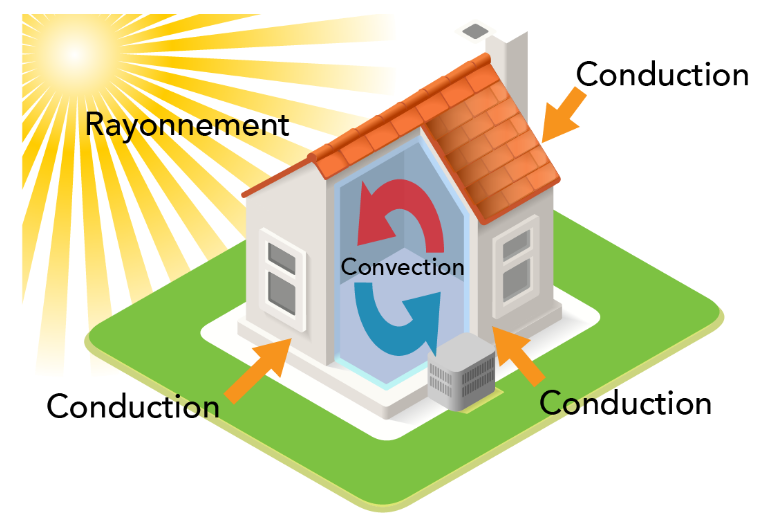
\includegraphics[width=0.4\linewidth]{modes_de_transfert.png}
	\caption{Différents modes de transfert thermique dans une maison. Source : poly de cours de Etienne Thibierge.}
\end{figure}

\subsubsection{Rayonnement}
\begin{definition}[Transfert thermique par rayonnement]
	On parle de transfert thermique par rayonnement lorsque l'énergie est transportée par des ondes électromagnétiques.
\end{definition}
C'est le cas, par exemple, d'un corps chaud qui perd de l'énergie en émettant un rayonnement conformément à la loi de Wien. Tous les corps perdent de l'énergie par rayonnement, mais les corps les plus chauds en perdent plus qu'ils n'en reçoivent, et c'est l'inverse pour les corps les plus froids. On en déduit que le transfert net d'énergie se fait bien des corps les plus chauds vers les corps les plus froids.

Le rayonnement d'un corps se fait en général dans le domaine de longueur d'onde de l'infrarouge thermique, autour de 10\,µm, sauf pour les corps très chauds comme le soleil ou une flamme, pour lesquels un rayonnement visible peut être émis (cf figure sur la température de flamme dans le cours de thermochimie).

\begin{remark}
	Ces transferts thermiques peuvent être quantifiés théoriquement à partir de l'intégrale spectrale de la loi de Planck, qui fournit la loi dite de Stefan-Boltzmann (cette loi n'est pas à connaître). Ce sont eux qui sont responsables de l'effet de serre et permettent d'expliquer le réchauffement climatique d'origine humaine.
\end{remark}

\subsubsection{Conduction}

\begin{definition}[Conduction]
	La conduction traduit un transfert thermique à travers un milieu matériel sans transport macroscopique de matière. Elle se fait de proche en proche par agitation thermique des particules.
\end{definition}

\begin{remark}
	Dans les solides cristallins, le phénomène de conduction peut être compris qualitativement à partir du modèle d'Einstein que nous avons vu dans le cours de thermodynamique statistique : lorsqu'un atome vibre, il va transmettre ses vibrations à ses voisins, ce qui va finir par agiter l'ensemble du solide cristallin et homogénéiser la température.
\end{remark}

\begin{figure}[htbp]
	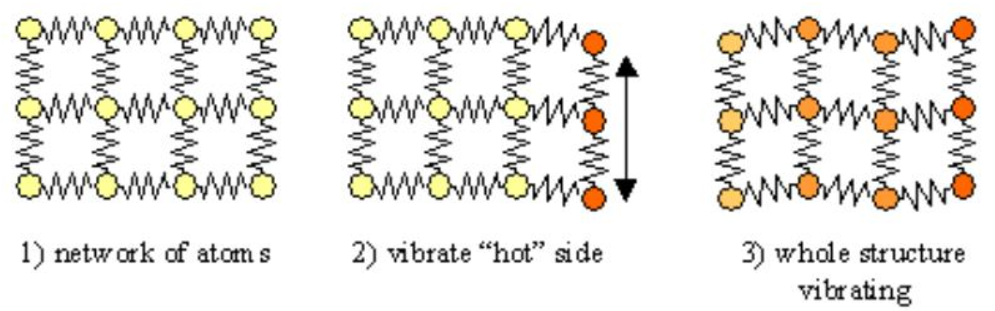
\includegraphics[width=0.8\linewidth]{conductivite_thermique_ressorts.png}
	\caption{Illustration du phénomène de conduction thermique dans un solide cristallin initialement à basse température, que l'on réchauffe par le côté droit. Source : Indian Institute of Technology Delhi.}
\end{figure}

La conduction est le mode de transfert thermique dominant dans les solides. Elle peut être décrite de manière locale, à travers une loi phénoménologique, appelée loi de Fourier :
\begin{theorem}[Loi de Fourier]
	Dans un milieu matériel, le vecteur densité de courant thermique par conduction est opposé et proportionnel au gradient de température :
	\begin{equation}
		\vv{j_{th,conduction}} = - \lambda \grad T
	\end{equation}
	où $\lambda$ est appelée la conductivité thermique du matériau. Elle se mesure en W$\cdot$m$^{-2} \cdot$K$^{-1}$.
	
	La loi de Fourier est valable uniquement :
	\begin{itemize}
		\item dans un solide isotrope (pas de direction privilégiée)
		\item si les gradients de température ne sont pas trop importants
		\item si les gradients de température ne varient pas trop rapidement
	\end{itemize} 
\end{theorem}

La loi de Fourier ne se démontre pas : il s'agit d'une loi phénoménologique fondée sur l'expérience. On peut citer quelques ordres de grandeur de conductivité thermique :
\begin{table}[htbp]
	\centering \begin{tabular}{lccccccc}
		\toprule
		Matériau & Cuivre & Zinc & Béton & Verre & Laine de verre & Eau & Air \\
		\midrule
		$\lambda$\,[W$\cdot$m$^{-2} \cdot$K$^{-1}$] & 400 & 100 & 1 & 0.9 & 0.05 & 0.6 & 0.03 \\
		\bottomrule
	\end{tabular}
\end{table}

\begin{capex}
	Interpréter la loi de Fourier à partir de cas limites (gradient faible ou fort). Comment est orienté le vecteur densité de flux thermique par rapport aux isothermes ? Commenter le signe $-$ présent dans la loi de Fourier.
\end{capex}

\begin{encart}[Matériaux très isolants]
	Afin d'optimiser la consommation énergétique des bâtiments, on cherche à construire des matériaux les plus isolants possibles sans être trop encombrants. Les solides cristallins ont l'avantage d'être résistants mais ils ont généralement une conductivité thermique trop élevée.
	
	Une équipe de recherche de l'université de Liverpool a récemment conçu un matériau très peu conducteur en exploitant sa structure cristalline : ils ont ajouté des couches d'atomes qui empêchent les vibrations de se propager dans le réseau cristallin, notamment en agissant sur la raideur des ressorts qui sont équivalents aux liaisons ioniques entre les différents ions. 
	
	Le solide obtenu, $\ce{Bi4O4SeCl2}$ a ainsi une conductivité thermique de seulement $0.1$\,W$\cdot$m$^{-1}\cdot$K$^{-1}$.
\end{encart}

\subsubsection{Convection}

\begin{definition}[Convection]
	Un transfert thermique par convection correspond à un transport net d'énergie thermique associé à un déplacement macroscopique de matière. Ce transfert est prédominant dans les fluides et généralement absent dans les solides.
\end{definition}

Très souvent, la convection trouve son origine dans les différences de densité induites par les différences de température dans un fluide : plus le fluide est chaud et plus sa densité est faible. Pour un gaz parfait, on a notamment l'expression suivante de la masse volumique : $\rho = \dfrac{M P}{RT}$ où $M$ est la masse molaire. Ainsi $\rho$ est bien une fonction décroissante de la température. Une bulle de gaz plus chaude va donc avoir tendance à s'élever, et une bulle de gaz plus froide à descendre. Des gradients de température vont donc se traduire par un déplacement macroscopique de matière.

\begin{proposition}
	Lorsqu'on a un transfert d'énergie thermique par convection dans un fluide, le fluide est en général bien mélangé si bien que la température y est relativement homogène.
\end{proposition}

\begin{figure}[htbp]
	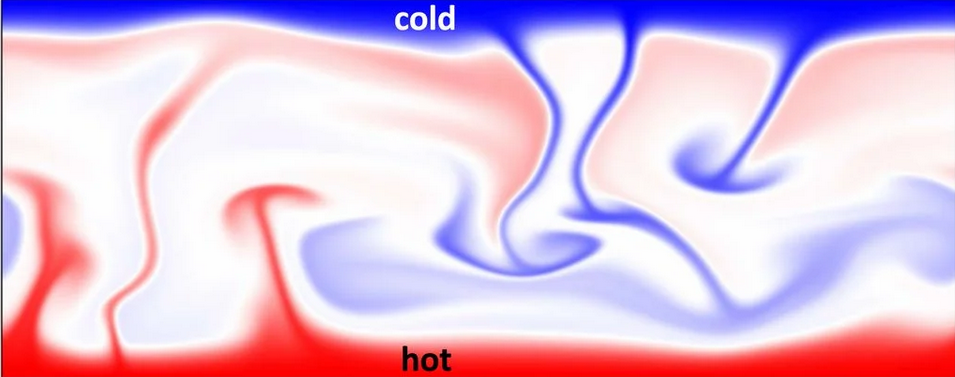
\includegraphics[width=0.8\linewidth]{convection.png}
	\caption{Simulation numérique de la convection dans un fluide chauffé par le bas (par exemple, cela pourrait être de l'eau dans une casserole). Les zones rouges indiquent des panaches chauds ascendants, et les zones bleues des panaches froids descendants. Source : Doering, C. R. (2020). \textit{Turning up the heat in turbulent thermal convection.} Proceedings of the National Academy of Sciences.}
\end{figure}

La convection joue par exemple un rôle important pour les transferts thermiques dans l'océan et dans l'atmosphère, ou bien à l'intérieur d'une maison. Elle permet aussi des transferts thermiques dans le manteau terrestre : bien que celui-ci soit solide, les échelles de temps sont suffisamment longues pour que les roches puissent se déplacer en raison de leur plasticité.

\paragraph{Transfert thermique conducto-convectif}

La convection joue aussi un rôle à l'interface entre un solide et un fluide : si le fluide est plus froid que le solide, il va extraire de l'énergie thermique du solide, et inversement. Par conservation de l'énergie, on a nécessairement continuité du flux thermique à une interface :
\begin{proposition}
	Le vecteur densité de courant thermique est une fonction continue de l'espace, y compris au niveau d'une interface.
\end{proposition}
En effet, on ne peut pas avoir une accumulation d'énergie au niveau de l'interface.

Le vecteur densité de courant thermique à l'interface est décrit phénoménologiquement par la loi de Newton :
\begin{theorem}
	Considérons une interface entre un solide et un fluide. On définit le vecteur unitaire $\vv n$ normal à la surface et orienté du solide vers le fluide. Alors à l'interface :
	\begin{equation}
		\vv{j_{th}} = h (T_{solide} - T_{fluide}) \vv n
	\end{equation}
	où $T_{fluide}$ et $T_{solide}$ sont les températures du fluide et du solide à l'interface, respectivement.
	$h$ est appelé le coefficient de transfert de la surface.
\end{theorem}
\begin{remark}
	En pratique, on constate que la valeur de $h$ dépend de nombreux paramètres, et en particulier de la vitesse d'écoulement du fluide, de l'état de surface du solide, de la nature du fluide et du solide.
\end{remark}

\begin{capex}
	On considère une interface de surface $S$ entre un fluide ($z>0$) et un solide ($z<0$). Quel est le mode de transfert thermique dans chacun des deux milieux ? Quelle est l'allure de la courbe de température $T(z)$ ?
	
	Déterminer l'expression du flux thermique $\Phi$ qui traverse l'interface de surface $S$, et relier le gradient de température $\frac{\dd T}{\dd z}(z=0^-)$ à la différence de température $T(z=0^+)-T(z=0^-)$.
\end{capex}


\section{Premier principe local dans un solide}

Nous avons décrit des lois locales permettant de décrire les transferts thermiques qui se produisent pour un champ de température donnée $T(M,t)$ à un instant $t$. Maintenant, nous souhaitons, en retour, savoir comment la température va varier en réponse au vecteur densité de courant thermique $\vv{j_{th}}$. Pour cela, nous avons besoin d'appliquer le premier principe.

\subsection{Cas d'un solide à une dimension}

Considérons le cas d'un solide de capacité thermique à pression constante $c_p$, dans lequel la température n'est fonction que d'une seule coordonnée cartésienne $x$. Nous appliquons le premier principe de la thermodynamique à un système fermé situé entre les coordonnées $x$ et $x+\dd x$, comme indiqué sur le schéma suivant :


\begin{capex}
	En supposant que l'on travaille à pression constante, établir l'expression du premier principe de la thermodynamique sous sa forme locale à une dimension. 
\end{capex}

\subsection{Equation locale de conservation de l'énergie ; opérateur divergence}

Considérons maintenant une situation à trois dimensions : on applique le premier principe à un volume élémentaire $\dd \tau = \dd x \dd y \dd z$. Alors, le transfert thermique reçu par le système pendant $\dd t$ est donné par :
\begin{align}
	\delta Q = \dd t \times ( &j_{th}^x(x)\dd y \dd z-j_{th}^x(x+\dd x)\dd y \dd z \\
	&+ j_{th}^y(y)\dd x \dd z-j_{th}^y(y+\dd y)\dd x \dd z \\
	&+ j_{th}^z(z)\dd x \dd y-j_{th}^z(z+\dd z)\dd x \dd y )
\end{align}
Ou encore, après simplification :
\begin{equation}
	\delta Q = \dd t \dd \tau \left( \frac{\partial j_{th}^x}{\partial x} + \frac{\partial j_{th}^y}{\partial y} + \frac{\partial j_{th}^z}{\partial z} \right)
\end{equation}

On constate que la puissance thermique volumique reçue par un élément du solide est proporionnelle à une fonction du vecteur densité de courant thermique que l'on appelle divergence :

\begin{definition}[Divergence]
	La divergence est un opérateur scalaire qui agit sur un champ vectoriel. Ainsi, en coordonnées cartésiennes, la divergence d'un champ $\vv A = (A_x,A_y,A_z)$ est définie par :
	\begin{equation}
		\div(\vv A) = \frac{\partial A_x}{\partial x} + \frac{\partial A_y}{\partial y} + \frac{\partial A_z}{\partial z}
	\end{equation}
\end{definition}

\begin{proposition}
	La divergence exprime la dispersion d'une grandeur (si elle est positive) ou la concentration de cette grandeur (si elle est négative) sous l'effet d'un champ de vecteurs caractérisant le flux de cette grandeur. 
\end{proposition}

Nous pouvons alors en déduire la forme générale du premier principe sous forme locale, en admettant l'effet d'un terme source de chaleur.

\begin{proposition}
	Considérons un solide de capacité thermique massique à pression constante $c_p$, siège de transferts thermiques caractérisés par une densité de courant thermique $\vv{j_{th}}$. Le premier principe de la thermodynamique sous sa forme locale peut alors s'écrire :
	\begin{equation}
		\mu c_p \frac{\partial T}{\partial t} + \div \vv{j_{th}} = 0
	\end{equation}
\end{proposition}

\begin{remark}
	On constate bien sur cette équation qu'une convergence de la densité de courant thermique ($\div \vv{j_{th}} <0$) va causer l'augmentation de la température, alors qu'une divergence de la densité de courant thermique ($\div \vv{j_{th}} > 0$) va causer une augmentation de la température.
\end{remark}

\subsection{Bilan macroscopique et théorème d'Ostrogradski}

Nous pouvons réaliser un bilan macroscopique pour interpréter plus facilement le résultat de ce bilan d'énergie. On considère ainsi un volume $\mathcal{V}$ fermé délimité par une surface $\Sigma$ que l'on oriente (comme en électrostatique) vers l'extérieur. 

\begin{capex}
	Appliquer le premier principe au volume $\mathcal{V}$. Obtenir une équation similaire en utilisant la loi locale de l'énergie, et commenter la différence entre les deux expressions obtenues.
\end{capex}

On constate que les deux lois obtenues ne sont pas tout à fait similaires, pourtant les deux expressions doivent être valides. Nous avons ainsi démontré que l'intégrale de la divergence d'un vecteur dans un volume fermé est reliée au flux de ce vecteur sur la surface délimitant ce volume : c'est le théorème d'Ostrogradski :
\begin{theorem}[Formule de Green-Ostrogradski]
	Soit $\vv A$ un champ vectoriel et $\mathcal{V}$ un volume fermé délimité par une surface $\Sigma$, alors :
	\begin{equation}
		\iiint_{\mathcal{V}} \div \vv A \dd \tau = \oiint_\Sigma \vv A \cdot \vv{\dd S}
	\end{equation}
\end{theorem}

\begin{remark}
	Cette formule vient conforter l'interprétation physique de la divergence : si la divergence de $\vv{j_{th}}$ est positive dans un volume fermé alors le flux de $\vv{j_{th}}$ sortant de ce volume est positif, c'est-à-dire que de l'énergie thermique sort de ce volume.
\end{remark}

\section{Diffusion thermique}

Nous avons maintenant :
\begin{itemize}
	\item Une description phénoménologique des transferts thermiques, qui nous donne la densité de courant thermique pour un champ de température donné ;
	\item Et la forme locale du premier principe, qui nous donne la variation temporelle de la température en réponse au champ de densité de courant thermique.
\end{itemize}

La combinaison de ces deux méthodes va nous permettre de déterminer l'équation d'évolution de la température dans le solide.

\subsection{Cas d'un solide à une dimension}

\begin{capex}
	Dans le cadre du modèle à une dimension, établir cette équation et montrer qu'elle est de la forme :
	\begin{equation}
		\frac{\partial T}{\partial t} = D \frac{\partial^2 T}{\partial x^2}
	\end{equation}
\end{capex}

Cette équation est une équation aux dérivées partielles d'ordre 1 en temps et d'ordre 2 en espace. On la nomme \textbf{équation de diffusion}. On remarque que l'équation n'est pas invariante par renversement du temps $t \to -t$, il s'agit donc d'une équation irréversible.

Pour le comprendre, nous pouvons remarquer que :
\begin{itemize}
	\item Dans les zones où la température est une fonction convexe de l'espace, on a tendance à avoir un minimum local de température. La température va avoir tendance à augmenter ;
	\item Au contraire, dans les zones où la température est une fonction concave de l'espace, on a un maximum local et la température va diminuer.
\end{itemize}
L'effet de cette équation est donc d'homogénéiser la température : on parle de diffusion thermique. Ceci est une conséquence directe du second principe de la thermodynamique, qui implique que les transferts thermiques se font spontanément du chaud vers le froid.

\subsection{Généralisation. Opérateur Laplacien.}

Nous pouvons désormais déterminer l'équation en trois dimensions. Pour cela, nous combinons la forme locale du permier principe avec la loi de Fourier pour obtenir l'équation suivante :
\begin{equation}
	\frac{\partial T}{\partial t} = D \div(\grad(T))
\end{equation}
Nous pouvons alors définir le laplacien d'une fonction :
\begin{definition}
	Le Laplacien est un opérateur scalaire qui agit sur un champ scalaire. Il se note $\Delta$ et est défini par :
	\begin{equation}
		\Delta A = \div(\grad(A))
	\end{equation}
\end{definition}

\begin{capex}
	Montrer qu'en coordonnées cartésiennes, le Laplacien d'une fonction vérifie :
	\begin{equation}
		\Delta A = \frac{\partial^2 A_x}{\partial x^2} + \frac{\partial^2 A_y}{\partial y^2} + \frac{\partial^2 A_z}{\partial z^2}
	\end{equation}
\end{capex}

Le laplacien d'un champ est une dérivée seconde de ce champ par rapport à l'espace, et est une mesure de sa convexité à plusieurs dimensions. Ainsi, on retrouve les mêmes propriétés que l'équation de diffusion à une dimension.

\begin{proposition}
	Dans un solide de capacité thermiqe massique $c_p$, de conductivité thermique $\lambda$ et de masse volumique $\mu$, la température obéti à l'équation de diffusion thermique :
	\begin{equation}
		\frac{\partial T}{\partial t} = D \Delta T
	\end{equation}
	où $D = \frac{\lambda}{\mu c_p}$.
\end{proposition}

\subsection{Diffusivité thermique}

\begin{definition}
	$D$ est appelée la diffusivité thermique du matériau. Elle se mesure en m$^2 \cdot$s$^{-1}$.
\end{definition}

Quelques valeurs caractéristiques sont données dans le tableau ci-dessous (elles ne sont pas à connaître) :
\begin{table}[htbp]
	\centering \begin{tabular}{lccccccc}
		\toprule
		Matériau & Cuivre & Zinc & Béton & Verre & Laine de verre & Eau & Air \\
		\midrule
		$D$\,[m$^2 \cdot$s$^{-1}$] & $10^{-4}$ & $4 \cdot 10^{-5}$ & $5 \cdot 10^{-7}$ & $5 \cdot 10^{-7}$ & $6 \cdot 10^{-7}$ & $10^{-7}$ & $2 \cdot 10^{-5}$ \\
		\bottomrule
	\end{tabular}
\end{table}

\begin{capex}
	A partir d'une analyse dimensionnelle de l'équation de diffusion, déterminer le temps caractéristique nécessaire pour atteindre l'équilibre thermique en fonction de la taille de l'échantillon.
\end{capex}

\section{Régime stationnaire unidimensionnel}

\subsection{Notion de résistance thermique}

On considère une paroi solide, d'épaisseur $e$ selon $\vv{e_x}$ et de section $S$, dans lequel la température ne dépend que d'une coordonnée $x$.

\begin{capex}
	En régime stationnaire, etablir la relation existant entre d'une part la différence de température $T_2 - T_1$ aux extrémités du solide en $x=0$ et $x=e$, et d'autre part le flux thermique $\Phi_{1 \to 2}$ traversant l'échantillon.
\end{capex}

\begin{definition}
	On définit la résistance thermique d'un échantillon solide $R_{th}$ comme le rapport entre la différence de température aux extrémités de l'échantillon, et le flux thermique qui le traverse en régime stationnaire :
	\begin{equation}
		T_1 - T_2 = R_{th} \Phi_{1 \to 2}
	\end{equation}
	Elle s'exprime en k$\cdot$W$^{-1}$.
	
	On définit également la conductance thermique $G_{th}$ par la relation inverse :
	\begin{equation}
		\Phi_{1 \to 2} = G_{th} (T_1 - T_2)
	\end{equation}
	On a alors :
	\begin{equation}
		G_{th} = \frac{1}{R_{th}}
	\end{equation}
\end{definition}

\begin{proposition}
	Pour un solide d'épaisseur $e$ et de section $S$ perpendiculaire à la direction du transfert thermique, on a :
	\begin{equation}
		R_{th} = \frac{e}{\lambda S}
	\end{equation}
\end{proposition}

\subsection{Analogie avec l'électrocinétique}

\begin{capex}
	Proposer une analogie avec la loi d'Ohm en électrocinétique.
	Parmi ces deux situations, lesquelles correspondent à des résistances thermiques en série et en parallèle ?
	\begin{itemize}
		\item Double vitrage.
		\item Deux vitres sur le même mur.
	\end{itemize}
	En déduire les lois d'association de résistances thermiques correspondantes.
\end{capex}



\end{document}
